%%%--- Example of usage of the lisings package
%%%--- Sarah Gerster, 24 Feb 2012
\documentclass[11pt,a4paper]{article}
\usepackage{graphicx}
\usepackage{texab}
\usepackage[utf8]{inputenc}

\begin{document}

\section{Include a figure generated with \Rp}
To include the figure generated with the \Rp function \texttt{pdf.latex()}
in the file \texttt{picture.R}, we use the \LaTeX{} command
\texttt{\textbackslash includegraphics\{\}}.

\begin{center}
  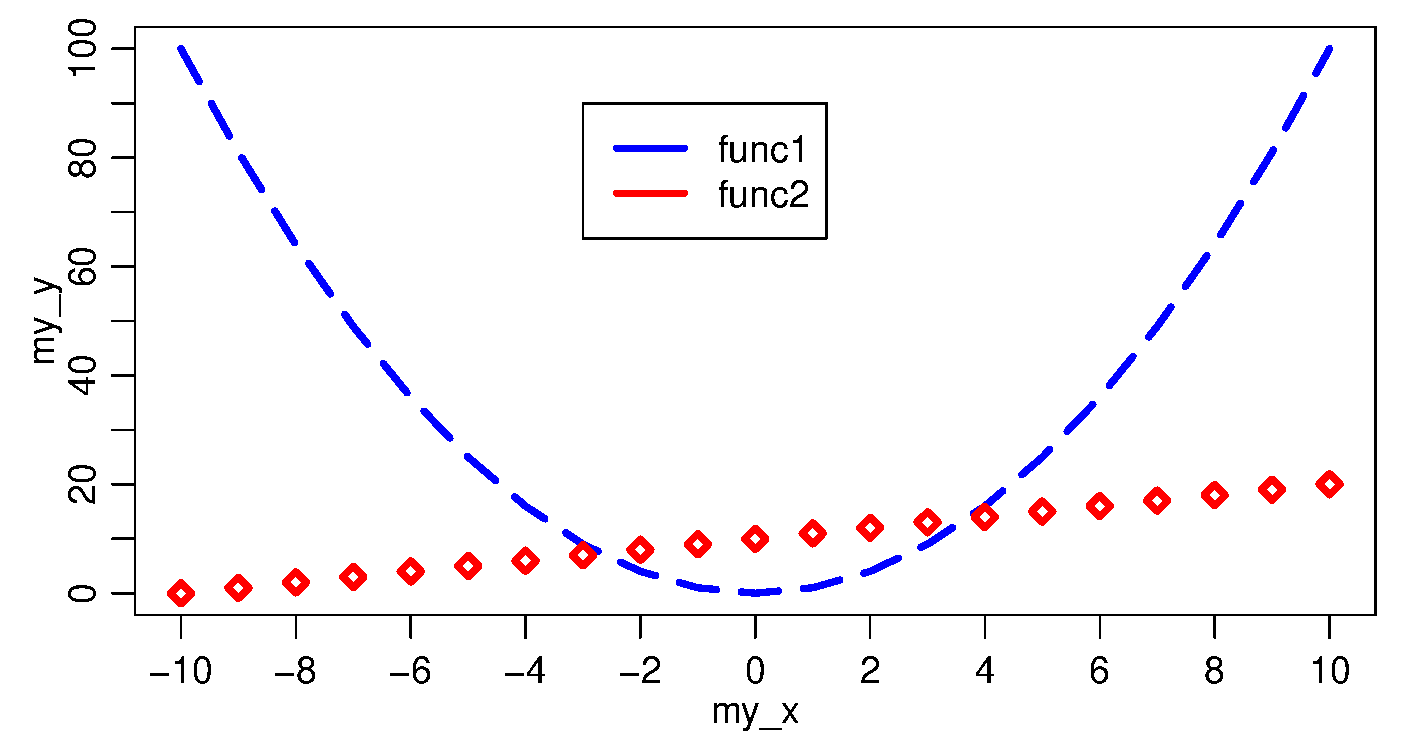
\includegraphics[width=0.9\textwidth]{test_plot}
\end{center}

By embedding the includegraphics in a \texttt{figure} environment, one can
also add a caption to the plot and reference it (see
Figure~\ref{fig:testfig}) easily. 

\begin{figure}[!h]
  \centering
  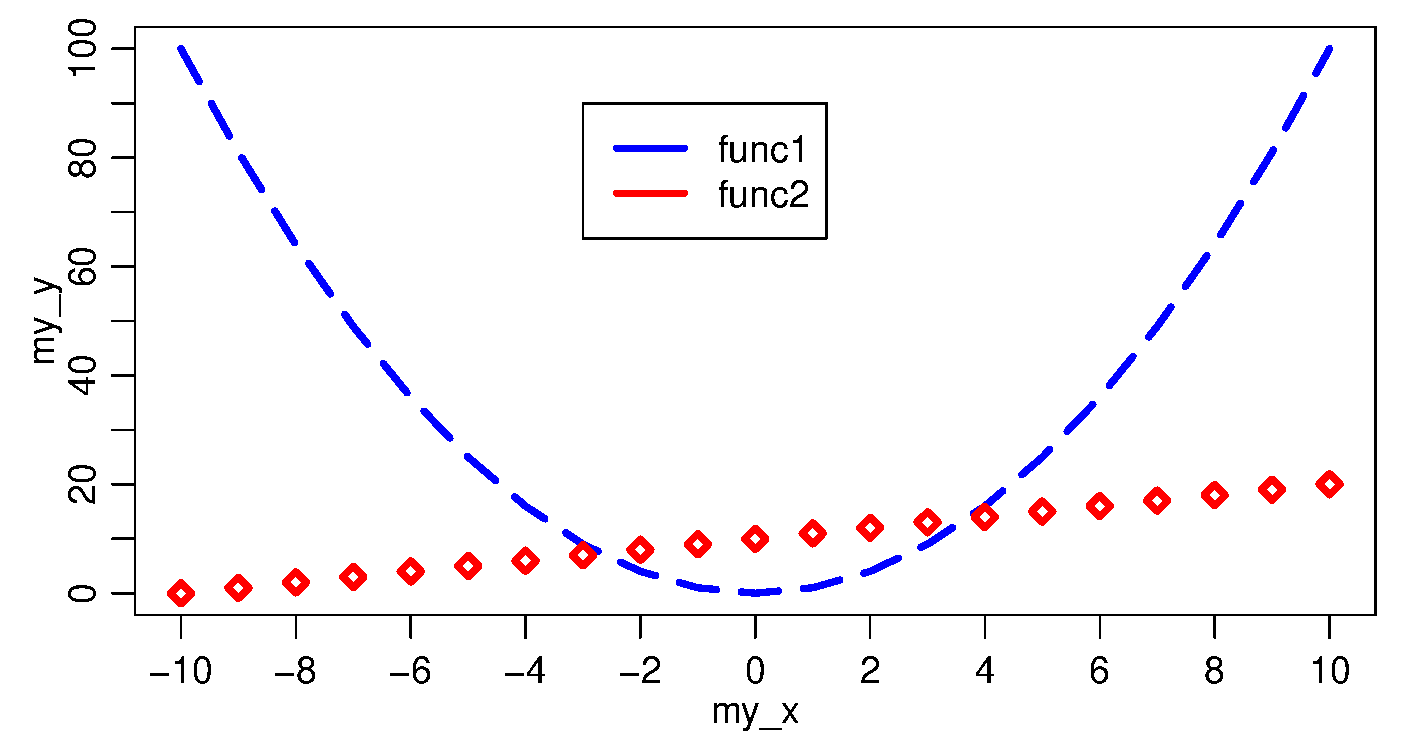
\includegraphics[width=0.9\textwidth]{test_plot}
  \label{fig:testfig}
  \caption{Simple plot to show how easily \Rp generated figures can be used
    in \LaTeX{}}
\end{figure}

\end{document}
